% Chapter 3

\chapter{Experimental Set Up} % Main chapter title

\label{Chapter3} % For referencing the chapter elsewhere, use \ref{Chapter3} 
In the interest of reproducibility we include in this section some of the considerations specific to our data set. Additionally we cover the data pre-processing steps taken prior to our experiments and describe our process for model tuning. Finally, we outline the procedure taken for the coherence testing, classification and clustering experiments. 

%----------------------------------------------------------------------------------------
\section{Data Considerations}

% THE DATASET
The data we used for our experiments comes from the August 2015 EPO Worldwide Patent Statistical Database (\keyword{PATSTAT}). According to the EPO, this data set contains over 90 million patent documents from leading industrialized and developing countries, with some documents as early as the nineteenth century. Thankfully, the expanse of this data is met with an equal level of documentation\footnote{For more information the official catalogue can be found at \url{http://goo.gl/LRQWnu}}. 


% CPC/IPC CLASSES
Due to time and computation limits, we ran experiments only on a subset of this data rather than the whole corpus. In order to break the PATSTAT into manageably sized subclasses we made use of Cooperative Patent Classification (\keyword{CPC}) labels. The CPC labels are a hierarchical system used globally to annotate patents according to the area of technology to which they relate. Predominantly we carried out our research on patents under the umbrella of \keyword{Y02E 10/20}, the subclass of patents relating to \keyword{hydro energy}. This subclass itself consisted of 5 smaller subsets of documents with more specific labels which we treated as true labels during our classification experiment, namely "Hydro energy", "Conventional", "Turbines and wheel", "Other parts", and "Stream and damless".

% PATENT FAMILIES
An additional consideration in filtering our data was the International Patent Documentation Centre \keyword{(INPADOC) patent family}. A patent family is a collection of patents filed in various countries to protect the same invention. We ensure that only one member of each patent family participates in the study so as not to 'double count' the same invention. Furthermore, only patents filed in English are considered. Figure \ref{fig:psqlSchema} contains the schema for the PostgreSQL database we constructed to hold relevant patent data.


\begin{figure}[h]
\centering
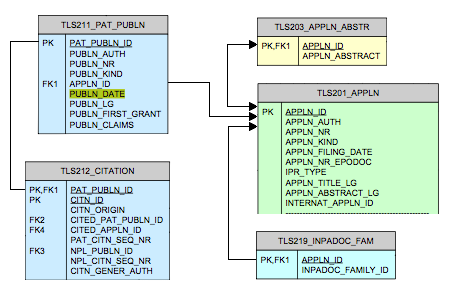
\includegraphics[width=130mm,scale=0.45]{Figures/psql_schema}
\decoRule
\caption[PSQLSchema]{Schema of PostgreSQL database containing relevant tables}
\label{fig:psqlSchema}
\end{figure}

% FORWARD CITATIONS
% how were forward citations calculated

% include  of subsetdatabase schema?
% stored in psql

\section{Data Pre-Processing}

%stopping, stemming, lower case, min_freq
The phrase "garbage in garbage out" is commonly used in machine learning to emphasize the importance of the data pre-processing step. We begin our pre-processing by retrieving abstracts from the aforementioned PSQL database and applying case folding such that words like "Turbine" at the beginning of a sentence will match the word "turbine" elsewhere. We then remove unnecessary symbols and punctuation via regex and apply stopping using the English \keyword{NLTK} stopwords list. This effectively removes common conjunctions and operational words from our corpus that don't actually contribute to the topics, such as "but, if, the, and" etc. 

\begin{tikzpicture}[node distance=4mm, >=latex',
 block/.style = {draw, rectangle, minimum height=10mm, minimum width=28mm,align=center},
rblock/.style = {draw, rectangle, rounded corners=0.5em},
tblock/.style = {draw, trapezium, minimum height=10mm, 
                 trapezium left angle=75, trapezium right angle=105, align=center},
                        ]
    \node [rblock]                   (a)     {Retrieve abstracts from PSQL};
    \node [block, right=of a]    (b)   {Tokenization, \\
	Regex cleaning $\&$ \\    
    Casefolding
    };
    \node [block, right=of b]   (c)  {Stopping};
    \node [block, below=1.2cm of a]  (d)      {Lemmatization};
    \node [block, right=of d]  (e)  {Frequency\\ Filtering};
    \node [tblock, right=of e]  (f)     {Serialize\\
    $\&$\\ Save};
    \node [coordinate, below right =.5cm and .5cm of c] (right) {}; 
    \node [coordinate, above left =.5cm and .5cm of d] (left) {}; 
    
    \path[draw,->] (a)      edge (b)
							 (b)      edge (c)
							 (c.east) -| (right) -- (left) |- (d)
							 (d)      edge (e)
							 (e)      edge (f)                    
                    ;
    \end{tikzpicture}

We then further distill the abstracts by applying lemmatization. This step is meant to reduce inflectional forms of a word such as "operates, operating, operational" to a base form "operate". After lemmatization, we remove any words occurring less than 25 times total, matching the implementation found in \parencite{Blei:2006:DTM:1143844.1143859}. Finally, we save the resulting corpus, totaling over 6,400 documents, and serialize the dictionary of vocabulary for subsequent access.

% number of unique words?

% used gensim, Python, Postgresql, ipython notebooks

\section{Tuning models}
\label{tuning}
The hyperparameters we select for our models can have a large influence on the topics that they infer. For this reason, prior to running any experiments, it is important to tune the hyperparameters of our topic models. The parameters we tuned specifically, were the number of topics $K$ and the maximum number of iterations $M_{iter}$. To do this we defined a range of values for these parameters and sampled parameter sets from this space uniformly. At each parameter set we evaluated the \keyword{umass}, \keyword{uci}, \keyword{npmi}, and \keyword{cv} topic coherence of the resulting model. 

In order to inspect the relationship our parameters had with topic coherence we visualized our results. Figure \ref{fig:DTMUCI} displays the c$\_$uci coherences of the DTM as a function of $K$ and $M_{iter}$. From this plot we can see that increasing the number of topics $K$ beyond a certain point fails to improve topic coherence with similar results for the number of iterations.

\begin{figure}[h]
\centering
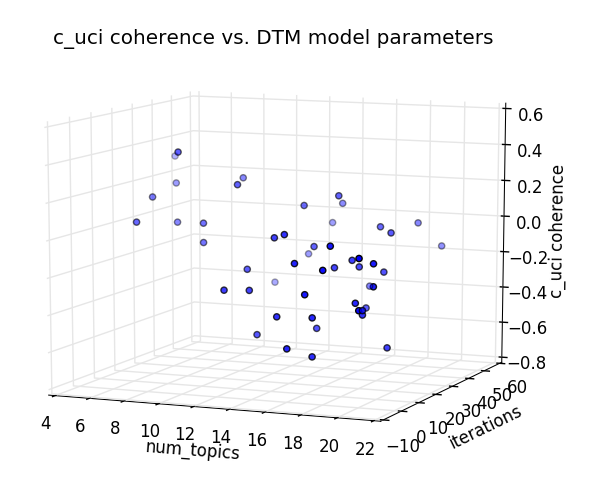
\includegraphics[width=130mm,scale=0.45]{Figures/uciCoherence}
\decoRule
\caption[DTMUCI]{c$\_$uci coherence scores for the DTM as a function of $K$ and $M_{iter}$}
\label{fig:DTMUCI}
\end{figure}

Table \ref{tab:paramtune} contains the best coherence scores obtained by each model for each measure after sampling our constrained parameter space. Despite tuning the models on a smaller set of documents it is interesting to note that a trend emerges, namely that the DTM tends to outperform both the DIM and the static LDA model in terms of topic coherence. However we reserve judgement until obtaining the final coherence testing results listed in section XXX. 

\begin{table}[ht]
\caption[HParamTuning]{The peak coherences achieved for various models and parameter choices.}
\label{tab:paramtune}
\centering
\begin{tabular}{l l l l l}
\toprule
\tabhead{Model} & \tabhead{c$\_$v} & \tabhead{c$\_$uci} & \tabhead{c$\_$npmi} & \tabhead{u$\_$mass} \\
\midrule
LDA & .4871 & .1455 & .0694 & -0.9813 \\
DTM & .5999 & .4098 & .1287 & -1.4496 \\ %.5916
DIM & .5789 & .1145 & .1175 & -1.6033 \\
\bottomrule\\
\end{tabular}
\end{table}

Though the optimal parameter sets suggested by each coherence measure did not greatly differ from one another, ultimately we selected the parameters recommended by the c$\_$v measure. We preferred the judgement of the c$\_$v measure as it is known to have the strongest correlation with human judgement \parencite{Roder:2015:EST:2684822.2685324}. The optimal parameter set found for the LDA model under the c$\_$v measure was $K$ = 13, $M_{iter}$ = 40, while for the DIM it was $K$ = 5, $M_{iter}$ = 32, and for the DTM it was $K$ = 17, $M_{iter}$ = 36. These were the parameters we used for the full scale coherence testing reported in section XXX.


%setting the alpha parameter in LDA as recommended by (e.g., as in Steyvers and Griffiths 2007) It acts as a form of regularization.
%A recommended setting is a = 50/K (Griffiths and Steyvers 2004; Steyvers and Griffiths 2007)

\section{Experimental Procedures}

\subsection{Coherence Testing}
% how we tested coherences of the models
The coherence testing experiment follows much the same procedure as above for hyperparameter tuning, with the difference being a full data set, and defined model parameters. We begin by training the LDA model, DTM and DIM over the same set of input documents belonging to the \keyword{Y02E 10/20} hydro energy CPC label, ranging from the year 1997 to 2015. Each model was trained under the optimal parameters found via the hyperparameter tuning process from section \ref{tuning}. 

Following model training, we retrieved all topics from the LDA model, DTM and the DIM, and assessed their semantic value via the \keyword{c$\_$v}, \keyword{c$\_$uci}, \keyword{c$\_$npmi}, and \keyword{U$\_$mass} coherence metrics. However because the DTM and DIM both output a \emph{series} of topics rather than a single set, the topic coherences were tested at each time step. Results for this experiment can be found in section XXX.

\subsection{Classification}
% how we classified 
To asses the efficacy of each model at creating feature vectors useful for document classification we begin by taking the same models as above, (the LDA model, DTM and DIM, trained on the hydro electric patents) and extract the document topic vectors for each document.

We then use 80$\%$ of these unsupervisedly learned feature vectors to train a collection of classifiers, and tested on the remaining 20$\%$ using the CPC subclasses for each document as true labels. We cross validated each classifier to ensure more robust estimates of performance, and selected the results of the classifier with the highest cross validated F1 score for each topic model. To further analyze the performance of each topic model's peak classifier we made use of the classification metrics outlined in section \ref{classificationmetrics} namely \keyword{accuracy}, \keyword{precision}, \keyword{recall}, and \keyword{F1 score}. Results for this experiment can be found in section XXX.


\subsection{Clustering}
% how we carried out clustering
Lastly, we conduct a clustering experiment to determine how well each model creates internally consistent groups of documents that are distinct from one another. We begin with the same set of models and data as with the other experiments, namely the LDA model, DTM and DIM trained on hydro electric PATSTAT patents. As with the classification experiment, we again extract the document topic vectors for each document.

However for this experiment, rather than beginning by handing the vectors to a series of classifiers, we begin by visualizing the space they formed using \keyword{TSNE}, \keyword{PCA}, and \keyword{MDS} embeddings to inspect the clusters by eye. After visually inspecting each model's document vectors we performed K-means clustering with $K=5$, (the number of true topics in the corpus). To evaluate clustering performance we feed the labels estimated by K-means for each set of document vectors, (alongside the respective true labels), to each of the clustering metrics outlined in section \ref{DocumentClustering}. These metrics include the \keyword{adjusted rand score}, \keyword{normalized mutual info}, \keyword{homogeneity}, \keyword{completeness} and \keyword{V-measure}. Results for this experiment can be found in section XXX.

